\section{Datasets}

In the course of this project, we used 3 different datasets:

\subsection{SurgToolLoc}
The dataset of the \emph{SurgToolLoc} Challenge is provided by the \emph{International Society for Computer Aided Surgery} (ISCAS). Its a result of surgical training exercises using the \emph{da Vinci} robotic system and contains \num{24695} video clips, each 30 seconds long, captured at a resolution of 1280$\times$720 pixels and 60fps, resulting in 1800 frames per video and almost 45 Million frames in total. Each video contains 3 out of 14 different tools (\ref{fig:surgtoolloc_tools}), of which not always every tool is active and visible, resulting in a certain amount of label errors. While this training dataset is only annotated with video-level tool labels, there exists a non-public test dataset additionally annotated with bounding boxes around the robotic tools. Sadly, we could not get access to this test dataset, which is why we will only test the tool classification on it and not the localization.

\begin{figure}[h]
	\centering
	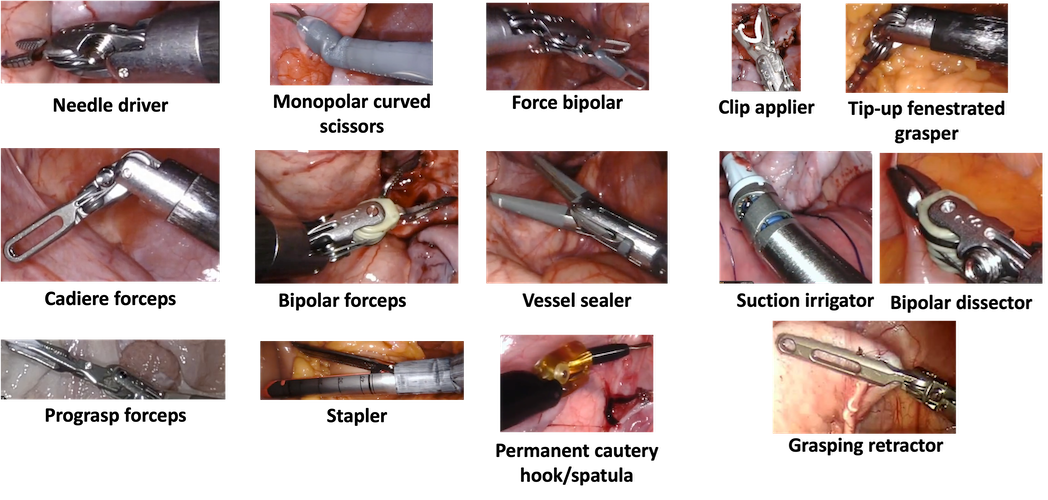
\includegraphics[width=15cm]{4_experiments/images/surgtoolloc_tools.png}
	\caption{All 14 tool classes of the \emph{SurgToolLoc} dataset.}
	\label{fig:surgtoolloc_tools}
\end{figure}

As training on such a massive dataset would have been unfeasible for our project, we created subset containing \num{10000} frames, randomly sampled from all videos and downscaled to 900$\times$620 pixels. \num{7000} of those frames were used for training and \num{3000} for testing. This re-sampling had the additional advantage of improving the extreme class-imbalance in the original data, where the most frequent class occurred \num{1000} times more often the least one (\ref{fig:surgtoolloc_tool_frequencies}).

\begin{figure}[h]
	\centering
	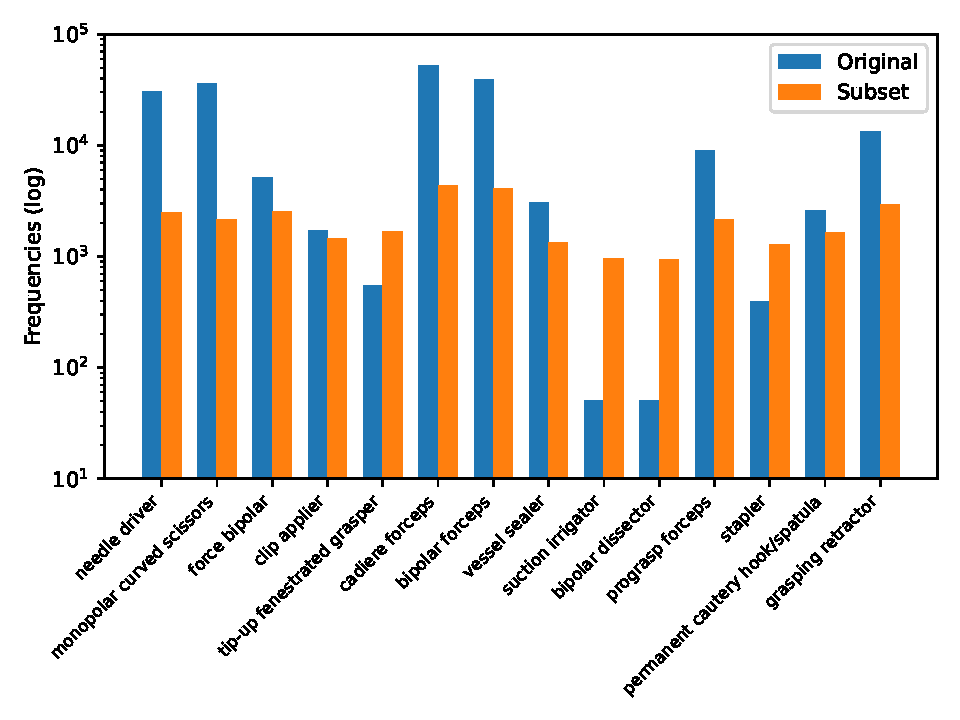
\includegraphics[width=15cm]{4_experiments/images/surgtoolloc_frequencies.pdf}
	\caption{Tool frequencies of the \emph{SurgToolLoc} dataset (video-level) and its subset (frame-level).}
	\label{fig:surgtoolloc_tool_frequencies}
\end{figure}

\subsection{Cholec80}
The \emph{Cholec80} dataset \cite{endonet} is provided by the \emph{CAMMA} research group at the University of Strasbourg and contains 80 videos of cholecystectomy surgeries, which combined result in about \num{180000} frames, most of them captured at resolution of 854$\times$480 pixels. It includes 7 different tool classes (\ref{fig:cholec80_tools}), from which a frame contains 0 to 3 and on average $1.32$ instances. In contrast to the \emph{SurgToolLoc} dataset, \emph{Cholec80} is annotated with frame-level tool labels, resulting in much less label errors. Bounding box labels were generated for the publication \cite{Vardazaryan}, but to our knowledge, have not been published.

\begin{figure}[h]
	\centering
	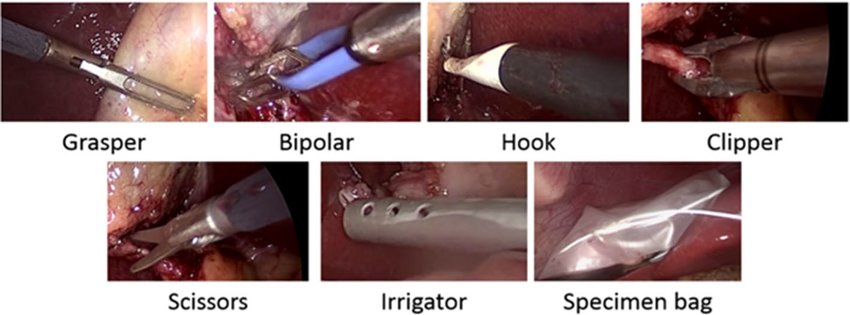
\includegraphics[width=13cm]{4_experiments/images/cholec80_tools.jpg}
	\caption{All 7 tool classes of the \emph{Cholec80} dataset.}
	\label{fig:cholec80_tools}
\end{figure}

Similar to before, this number of frames would have been unmanageable for us, so we again created a subset, of this time 6000 frames, randomly sampled from all classes. While in the original set, the factor between the least and most appearing tool is about 30, it's only 4.5 in the subset. A complete class-balance would be hard to achieve, as some of the tools, like the Grasper, almost exclusively are used with the other tools together.


\subsection{M2CAI16}

The \emph{M2CAI16} dataset contains \num{2811} frames (\num{2248} for training and \num{563} for testing) gathered from the videos 61-76 in \emph{Cholec80}. Every frame is fully annotated with tool presence labels and bounding boxes. Its size makes it manageable for us and its bounding box annotations can be used to evaluate the tool localization, which is why we will mainly use it for the following experiments.


\begin{figure}[h]
	\makebox[\linewidth][c]{
		\begin{subfigure}[b]{.6\textwidth}
			\centering
			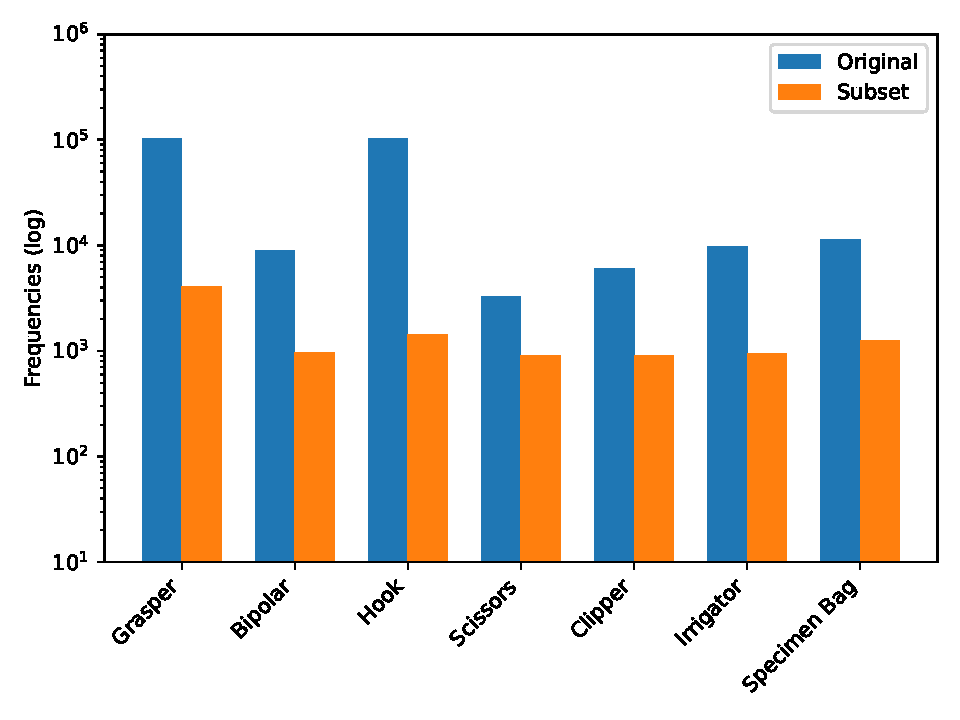
\includegraphics[width=9cm]{4_experiments/images/cholec_frequencies.pdf}
			\label{fig:cholec80_frequncies}
		\end{subfigure}%
		\begin{subfigure}[b]{.6\textwidth}
			\centering
			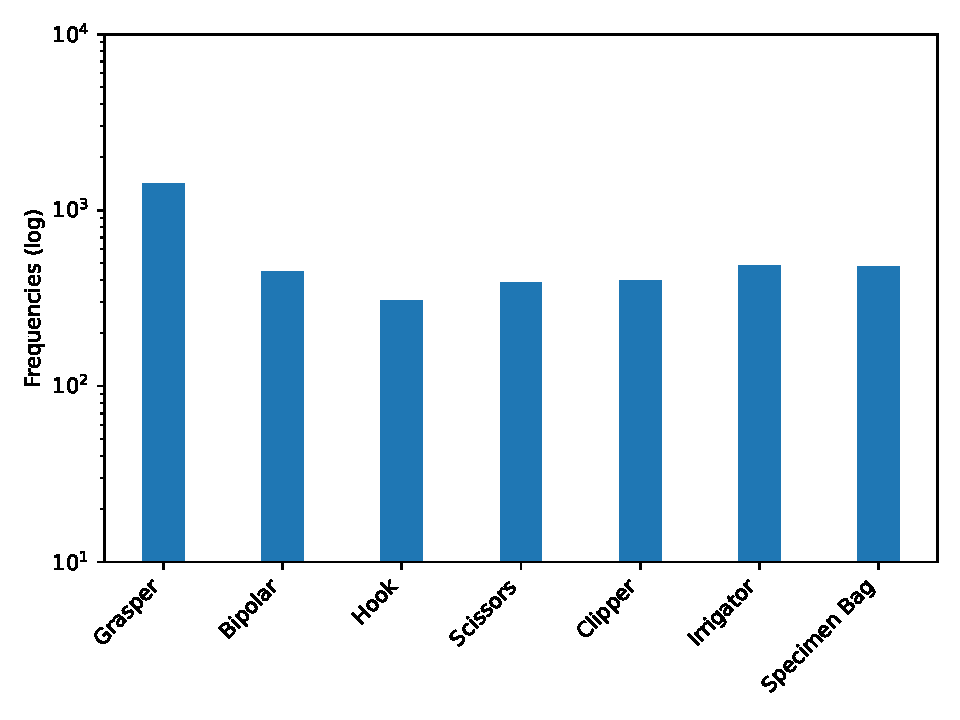
\includegraphics[width=9cm]{4_experiments/images/m2cai16_frequencies.pdf}
			\label{fig:m2cai16_frequencies}
		\end{subfigure}
	}
	\caption{(left) Frame-level tool frequencies of the \emph{Cholec80} dataset and its subset \\(right) Frame-level tool frequencies of the \emph{M2CAI16} dataset}
\end{figure}